    In Einstein’s theory, time is defined operationally through the arrival and departure of light signals. Simultaneity is not absolute, but constructed by coordinating photon trajectories between clocks. This makes time a relational concept—dependent on the motion of observers and the invariance of light speed.

    \begin{table}[h!]
        \centering
        \begin{tabular}{|c|c|c|c|}
            \hline
            \textbf{Theory} & \textbf{Time} & \textbf{Simultaneity} & \textbf{Defined By} \\
            \hline
            Newton & Absolute & Universal & External flow of time \\
            Einstein (SR/GR) & Relative & Frame-dependent & Light signal coordination \\
            VAM & Layered (N, $\tau$, $S(t)$) & Phase-coherent & Vortex swirl phase $\Omega(r)$ \\
            \hline
        \end{tabular}
        \caption{Comparison of time and simultaneity in Newtonian, Einsteinian, and VAM frameworks.}
    \end{table}

    In contrast, the Vortex Æther Model grounds time in the internal dynamics of the medium itself. Absolute æther time \( N \) flows uniformly, while local time \( \tau \) and swirl clock time \( S(t) \) emerge from the rotational energy and helicity of vortex structures. Simultaneity is no longer a matter of synchronization via photons—it is encoded in the shared phase coherence of knotted circulation. In this sense, VAM replaces relativistic light-clock simultaneity with a topologically grounded, energetically conserved temporal ontology.



\resizebox{\textwidth}{!}{%
      \centering
    \scriptsize
        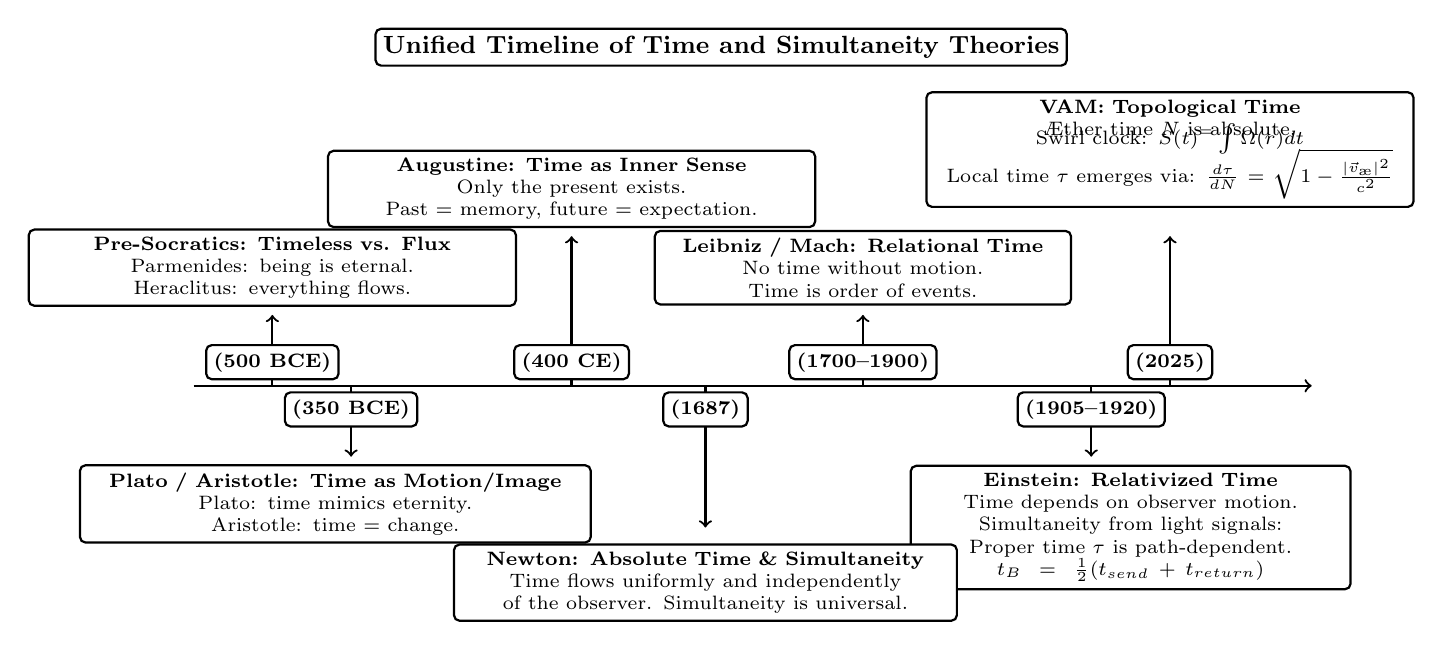
\begin{tikzpicture}
        \scriptsize
        % Timeline base
        \draw[->, thick] (-1,0) -- (13.2,0);

        % Arrows above timeline (short, as requested)
        \draw[->, thick] (0,0) -- (0,0.9);       % Pre-Socratics
        \draw[->, thick] (3.8,0) -- (3.8,1.9);   % Augustine
        \draw[->, thick] (7.5,0) -- (7.5,0.9);   % Einstein
        \draw[->, thick] (11.4,0) -- (11.4,1.9); % VAM

        % Arrows below timeline (short, as requested)
        \draw[->, thick] (1.0,0) -- (1.0,-0.9);     % Plato/Aristotle
        \draw[->, thick] (5.5,0) -- (5.5,-1.8);     % Newton
        \draw[->, thick] (10.4,0) -- (10.4,-0.9);     % Leibniz/Mach

            %--- Root title cards (above timeline) ---
        \node[draw, thick, rounded corners=2pt, fill=white, align=center, font=\bfseries ] at (0, .3)   {(500 BCE)};
        \node[draw, thick, rounded corners=2pt, fill=white, align=center, font=\bfseries ] at (3.8, .3) {(400 CE)};
        \node[draw, thick, rounded corners=2pt, fill=white, align=center, font=\bfseries ] at (7.5, .3) {(1700--1900)};
        \node[draw, thick, rounded corners=2pt, fill=white, align=center, font=\bfseries ] at (11.4, .3){(2025)};

        %--- Root title cards (below timeline) ---
        \node[draw, thick, rounded corners=2pt, fill=white, align=center, font=\bfseries ] at (1.0,- .3) {(350 BCE)};
        \node[draw, thick, rounded corners=2pt, fill=white, align=center, font=\bfseries ] at (5.5,- .3) {(1687)};
        \node[draw, thick, rounded corners=2pt, fill=white, align=center, font=\bfseries ] at (10.4,- .3) {(1905--1920)};

            % Timeline label
        \node[draw, thick, fill=white, rounded corners=2pt, font=\small] at (5.7,4.3) {\textbf{Unified Timeline of Time and Simultaneity Theories}};

        % --- Pre-Socratics ---
        \node[draw, rounded corners=2pt, thick, align=center, fill=white, text width=6cm] at (0,1.5) {
        \textbf{Pre-Socratics: Timeless vs. Flux} \\% [-0.8em]
        Parmenides: being is eternal. \\% [-0.8em]
        Heraclitus: everything flows.
        };

        % --- Augustine ---
        \node[draw, rounded corners=2pt, thick, align=center, fill=white, text width=6cm] at (3.8,2.5) {
        \textbf{Augustine: Time as Inner Sense} \\% [-0.8em]
        Only the present exists. \\% [-0.8em]
        Past = memory, future = expectation.
        };

        % --- Leibniz / Mach ---
        \node[draw, rounded corners=2pt, thick, align=center, fill=white, text width=5.1cm] at (7.5,1.5) {
        \textbf{Leibniz / Mach: Relational Time} \\% [-0.8em]
        No time without motion. \\% [-0.8em]
        Time is order of events.
        };
        % --- VAM (modern) ---
        \node[draw, rounded corners=2pt, thick, align=center, fill=white, text width=6.0cm] at (11.4,3.0) {
        \textbf{VAM: Topological Time} \\% [-0.8em]
        Æther time $N$ is absolute. \\[-0.6em]
        Swirl clock: $S(t)^\circlearrowleft = \int \Omega(r) dt$ \\[-0.4em]
        Local time $\tau$ emerges via: $ \frac{d\tau}{dN} = \sqrt{1 - \frac{|\vec{v}_\text{\ae}|^2}{c^2}}$

        };


        % --- Plato / Aristotle ---
        \node[draw, rounded corners=2pt, thick, align=center, fill=white, text width=6.3cm] at (0.8,-1.5) {
        \textbf{Plato / Aristotle: Time as Motion/Image} \\% [-0.8em]
        Plato: time mimics eternity. \\% [-0.8em]
        Aristotle: time = change.
        };



        % --- Einstein ---
        \node[draw, rounded corners=2pt, thick, align=center, fill=white, text width=5.4cm] at (10.9,-1.8) {
        \textbf{Einstein: Relativized Time} \\% [-0.8em]
        Time depends on observer motion. \\% [-0.8em]
        Simultaneity from light signals: \\% [-0.8em]
        Proper time $\tau$ is path-dependent.\\% [-0.8em]
        $t_B = \frac{1}{2}(t_{\text{send}} + t_{\text{return}})$
        };

        % --- Newton ---
        \node[draw, rounded corners=2pt, thick, align=center, fill=white, text width=6.2cm] at (5.5,-2.5) {
        \textbf{Newton: Absolute Time \& Simultaneity} \\% [-0.8em]
        Time flows uniformly and independently \\% [-0.8em]
        of the observer. Simultaneity is universal.
        };
         \end{tikzpicture}
        \caption{\textbf{Chronology of simultaneity theories across physics and philosophy.} From ancient views of time as change or inner sense, through Newton’s absolute simultaneity and Einstein’s frame-dependent proper time, to VAM’s swirl-based causal layering. The model introduces a physically grounded sequence of time variables culminating in measurable, observer-dependent time ($\tau$) and topological time ($\mathbb{K}$).}\label{fig:history-time-simultaneity}
}

\begin{center}
\footnotesize
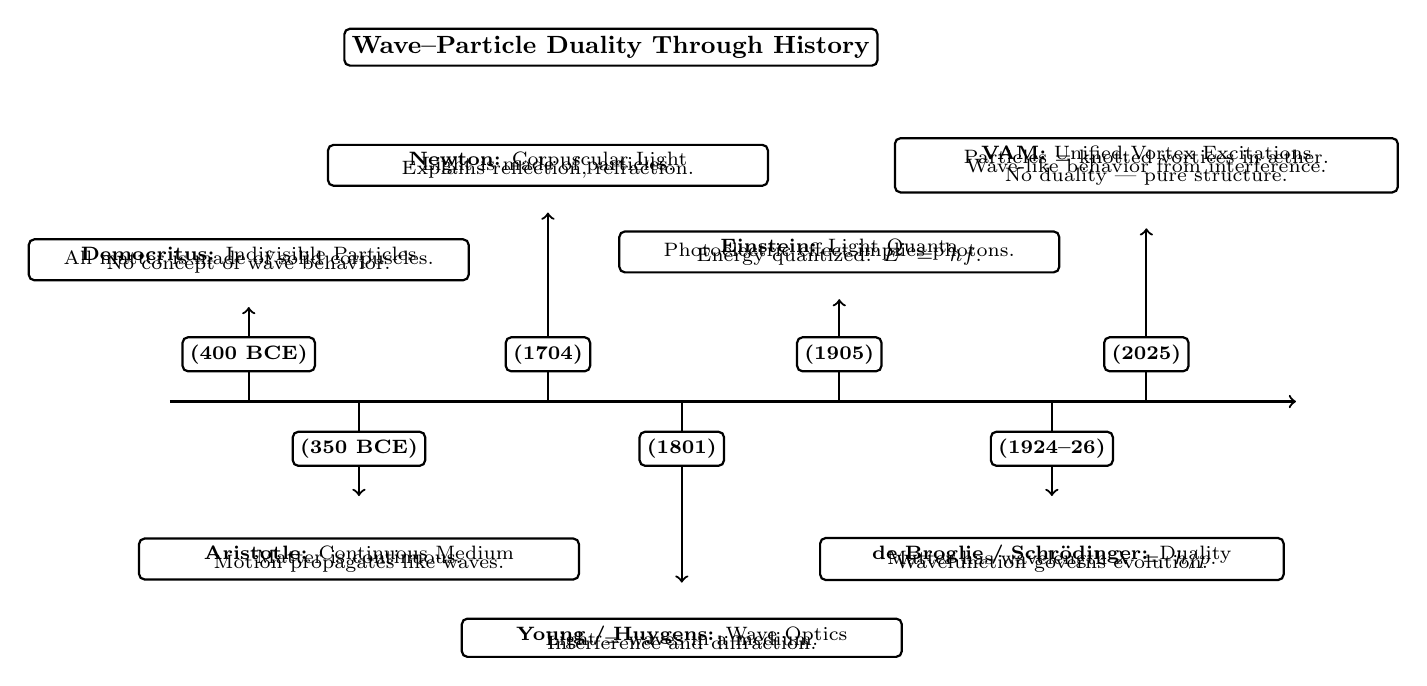
\begin{tikzpicture}
\scriptsize

% Timeline base
\draw[->, thick] (-1,0) -- (13.3,0);

% Arrows above timeline
\draw[->, thick] (0,0) -- (0,1.2);       % Democritus
\draw[->, thick] (3.8,0) -- (3.8,2.4);   % Newton
\draw[->, thick] (7.5,0) -- (7.5,1.3);   % Einstein
\draw[->, thick] (11.4,0) -- (11.4,2.2); % VAM

% Arrows below timeline
\draw[->, thick] (1.4,0) -- (1.4,-1.2);     % Aristotle
\draw[->, thick] (5.5,0) -- (5.5,-2.3);     % Young/Huygens
\draw[->, thick] (10.2,0) -- (10.2,-1.2);   % de Broglie

% --- Date labels ---
\node[draw, thick, rounded corners=2pt, fill=white, align=center, font=\bfseries ] at (0, .6)   {(400 BCE)};
\node[draw, thick, rounded corners=2pt, fill=white, align=center, font=\bfseries ] at (3.8, .6) {(1704)};
\node[draw, thick, rounded corners=2pt, fill=white, align=center, font=\bfseries ] at (7.5, .6) {(1905)};
\node[draw, thick, rounded corners=2pt, fill=white, align=center, font=\bfseries ] at (11.4, .6){(2025)};

\node[draw, thick, rounded corners=2pt, fill=white, align=center, font=\bfseries ] at (1.4,- .6) {(350 BCE)};
\node[draw, thick, rounded corners=2pt, fill=white, align=center, font=\bfseries ] at (5.5,- .6) {(1801)};
\node[draw, thick, rounded corners=2pt, fill=white, align=center, font=\bfseries ] at (10.2,- .6) {(1924--26)};

% Timeline label
\node[draw, thick, fill=white, rounded corners=2pt, font=\small] at (4.6,4.5) {\textbf{Wave–Particle Duality Through History}};

% --- Democritus ---
\node[draw, rounded corners=2pt, thick, align=center, fill=white, text width=5.4cm] at (0,1.8) {
\textbf{Democritus:} Indivisible Particles \\[-0.8em]
All matter is made of solid corpuscles. \\[-0.8em]
No concept of wave behavior.
};

% --- Newton ---
\node[draw, rounded corners=2pt, thick, align=center, fill=white, text width=5.4cm] at (3.8,3.0) {
\textbf{Newton:} Corpuscular Light \\[-0.8em]
Light is made of particles. \\[-0.8em]
Explains reflection, refraction.
};

% --- Einstein ---
\node[draw, rounded corners=2pt, thick, align=center, fill=white, text width=5.4cm] at (7.5,1.9) {
\textbf{Einstein:} Light Quanta \\[-0.8em]
Photoelectric effect implies photons. \\[-0.8em]
Energy quantized: \( E = hf \).
};

% --- VAM ---
\node[draw, rounded corners=2pt, thick, align=center, fill=white, text width=6.2cm] at (11.4,3.0) {
\textbf{VAM:} Unified Vortex Excitations \\[-0.8em]
Particles = knotted vortices in æther. \\[-0.6em]
Wave-like behavior from interference. \\[-0.6em]
No duality — pure structure.
};

% --- Aristotle ---
\node[draw, rounded corners=2pt, thick, align=center, fill=white, text width=5.4cm] at (1.4,-2.0) {
\textbf{Aristotle:} Continuous Medium \\[-0.8em]
Matter is continuous. \\[-0.8em]
Motion propagates like waves.
};

% --- Young / Huygens ---
\node[draw, rounded corners=2pt, thick, align=center, fill=white, text width=5.4cm] at (5.5,-3.0) {
\textbf{Young / Huygens:} Wave Optics \\[-0.8em]
Light = waves in a medium. \\[-0.8em]
Interference and diffraction.
};

% --- de Broglie / Schrödinger ---
\node[draw, rounded corners=2pt, thick, align=center, fill=white, text width=5.7cm] at (10.2,-2.0) {
\textbf{de Broglie / Schrödinger:} Duality \\[-0.8em]
Matter has wavelength \( \lambda = h/p \). \\[-0.8em]
Wavefunction governs evolution.
};

\end{tikzpicture}
\captionof{figure}{Development of wave–particle duality: from atomistic corpuscles and wave optics, through quantum superposition, to VAM’s unified vortex excitation model.}
\end{center}
\begin{center}
\footnotesize
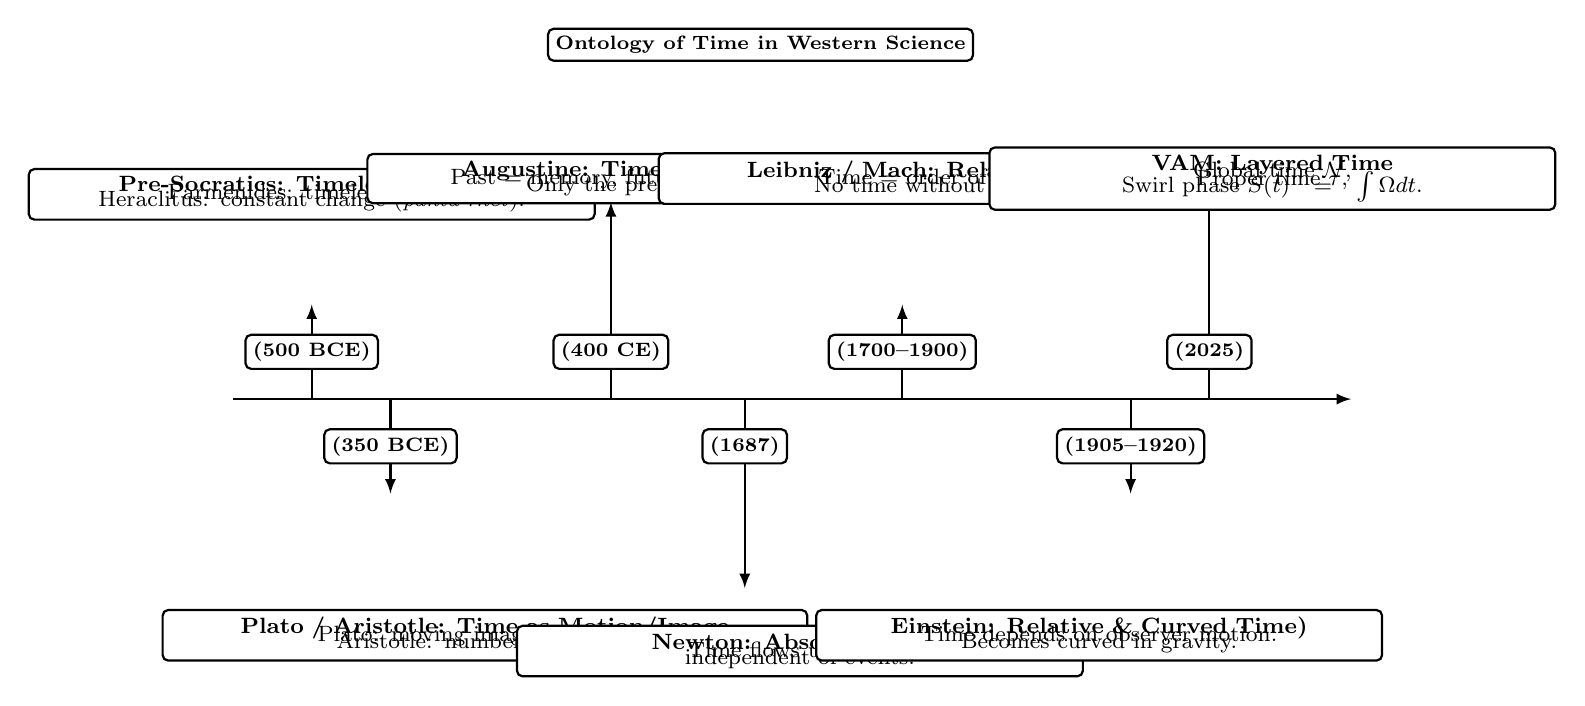
\begin{tikzpicture}[node distance=3.5cm, every node/.style={font=\footnotesize}, >=latex]
\scriptsize


% Timeline base
\draw[->, thick] (-1,0) -- (13.2,0);

% Arrows above timeline (short, as requested)
\draw[->, thick] (0,0) -- (0,1.2);       % Pre-Socratics
\draw[->, thick] (3.8,0) -- (3.8,2.5);   % Augustine
\draw[->, thick] (7.5,0) -- (7.5,1.2);   % Einstein
\draw[->, thick] (11.4,0) -- (11.4,3.0); % VAM

% Arrows below timeline (short, as requested)
\draw[->, thick] (1.0,0) -- (1.0,-1.2);     % Plato/Aristotle
\draw[->, thick] (5.5,0) -- (5.5,-2.4);     % Newton
\draw[->, thick] (10.4,0) -- (10.4,-1.2);     % Leibniz/Mach

    %--- Root title cards (above timeline) ---
\node[draw, thick, rounded corners=2pt, fill=white, align=center, font=\bfseries ] at (0, .6)   {(500 BCE)};
\node[draw, thick, rounded corners=2pt, fill=white, align=center, font=\bfseries ] at (3.8, .6) {(400 CE)};
\node[draw, thick, rounded corners=2pt, fill=white, align=center, font=\bfseries ] at (7.5, .6) {(1700--1900)};
\node[draw, thick, rounded corners=2pt, fill=white, align=center, font=\bfseries ] at (11.4, .6){(2025)};

%--- Root title cards (below timeline) ---
\node[draw, thick, rounded corners=2pt, fill=white, align=center, font=\bfseries ] at (1.0,- .6) {(350 BCE)};
\node[draw, thick, rounded corners=2pt, fill=white, align=center, font=\bfseries ] at (5.5,- .6) {(1687)};
\node[draw, thick, rounded corners=2pt, fill=white, align=center, font=\bfseries ] at (10.4,- .6) {(1905--1920)};

% Label (centered box)
\node[draw, thick, fill=white, rounded corners=2pt, font=\scriptsize] at (5.7,4.5) {\textbf{Ontology of Time in Western Science}};

% Ancient Greek: Parmenides / Heraclitus
\node[draw, rounded corners=2pt, thick, align=center, fill=white, text width=7cm] at (0,2.6) {
\textbf{Pre-Socratics: Timeless vs. Flux}  \\[-0.8em]
Parmenides: timeless being.  \\[-0.8em]
Heraclitus: constant change (\textit{panta rhei}).
};

% Plato / Aristotle
\node[draw, rounded corners=2pt, thick, align=center, fill=white, text width=8cm] at (2.2,-3.0) {
\textbf{Plato / Aristotle: Time as Motion/Image}  \\[-0.8em]
Plato: moving image of eternity.  \\[-0.8em]
Aristotle: number of change.
};

% Augustine
\node[draw, rounded corners=2pt, thick, align=center, fill=white, text width=7cm] at (4.3,2.8) {
\textbf{Augustine: Time as Inner Sense}  \\[-0.8em]
Past = memory, future = anticipation.  \\[-0.8em]
Only the present is real.
};

% Newton
\node[draw, rounded corners=2pt, thick, align=center, fill=white, text width=7cm] at (6.2,-3.2) {
\textbf{Newton: Absolute Time)}  \\[-0.8em]
Time flows uniformly,  \\[-0.8em]
independent of events.
};


% Relationalists: Leibniz / Mach
\node[draw, rounded corners=2pt, thick, align=center, fill=white, text width=7cm] at (8.0,2.8) {
\textbf{Leibniz / Mach: Relational Time}  \\[-0.8em]
Time = order of events.  \\[-0.8em]
No time without change.
};

% Einstein
\node[draw, rounded corners=2pt, thick, align=center, fill=white, text width=7cm] at (10.0,-3.0) {
\textbf{Einstein: Relative \& Curved Time)}  \\[-0.8em]
Time depends on observer motion.  \\[-0.8em]
Becomes curved in gravity.
};


% VAM
\node[draw, rounded corners=2pt, thick, align=center, fill=white, text width=7cm] at (12.2,2.8) {
\textbf{VAM: Layered Time}  \\[-0.8em]
Global time \( \mathcal{N} \),  \\[-0.8em]
Proper time \( \tau \),  \\[-0.8em]
Swirl phase \( S(t) = \int \Omega dt \).
};


\end{tikzpicture}
\captionof{figure}{Historical evolution of temporal ontology: from pre-Socratic polarity to Einstein's spacetime and the layered temporality of the Vortex Æther Model.}
\end{center}
\begin{center}
\footnotesize
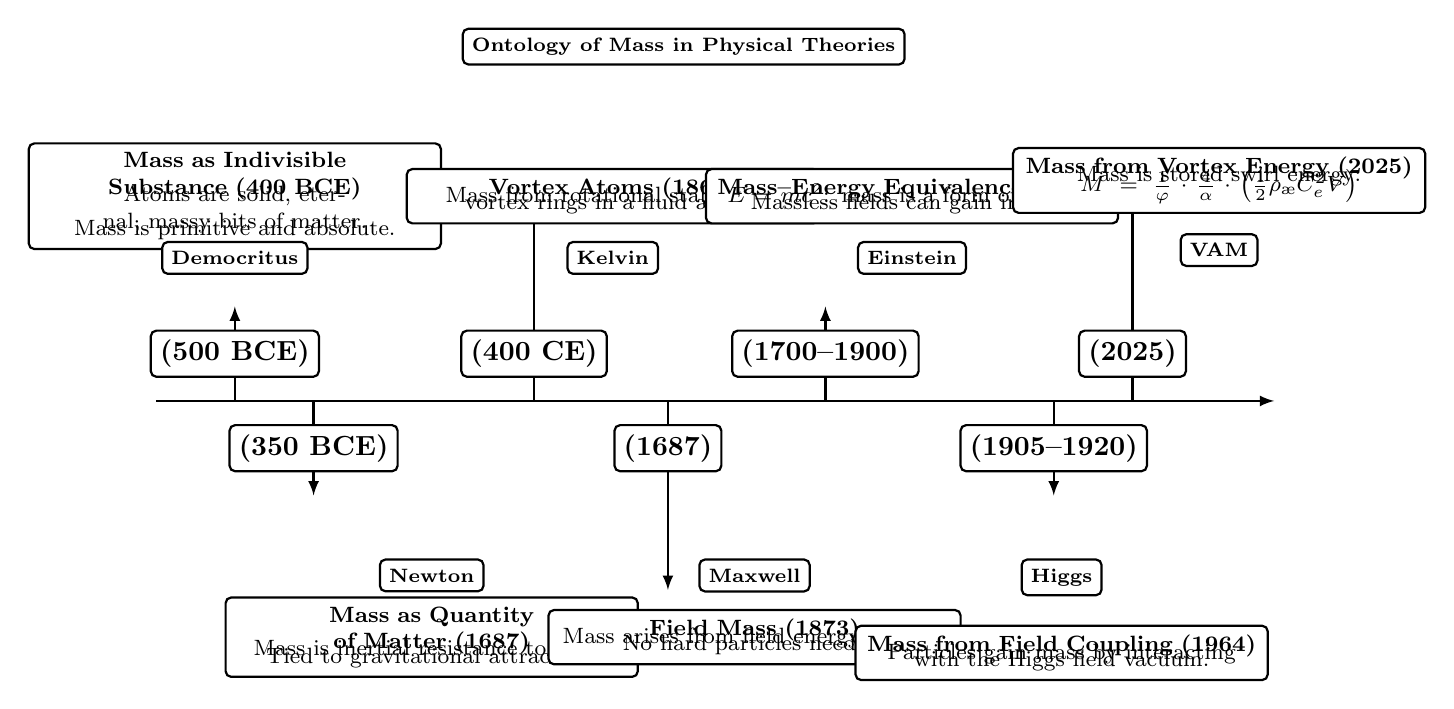
\begin{tikzpicture}[node distance=3.5cm, every node/.style={font=\footnotesize}, >=latex]


% Timeline base
\draw[->, thick] (-1,0) -- (13.2,0);

% Arrows above timeline (short, as requested)
\draw[->, thick] (0,0) -- (0,1.2);       % Pre-Socratics
\draw[->, thick] (3.8,0) -- (3.8,2.5);   % Augustine
\draw[->, thick] (7.5,0) -- (7.5,1.2);   % Einstein
\draw[->, thick] (11.4,0) -- (11.4,3.0); % VAM

% Arrows below timeline (short, as requested)
\draw[->, thick] (1.0,0) -- (1.0,-1.2);     % Plato/Aristotle
\draw[->, thick] (5.5,0) -- (5.5,-2.4);     % Newton
\draw[->, thick] (10.4,0) -- (10.4,-1.2);     % Leibniz/Mach

    %--- Root title cards (above timeline) ---
\node[draw, thick, rounded corners=2pt, fill=white, align=center, font=\bfseries ] at (0, .6)   {(500 BCE)};
\node[draw, thick, rounded corners=2pt, fill=white, align=center, font=\bfseries ] at (3.8, .6) {(400 CE)};
\node[draw, thick, rounded corners=2pt, fill=white, align=center, font=\bfseries ] at (7.5, .6) {(1700--1900)};
\node[draw, thick, rounded corners=2pt, fill=white, align=center, font=\bfseries ] at (11.4, .6){(2025)};

%--- Root title cards (below timeline) ---
\node[draw, thick, rounded corners=2pt, fill=white, align=center, font=\bfseries ] at (1.0,- .6) {(350 BCE)};
\node[draw, thick, rounded corners=2pt, fill=white, align=center, font=\bfseries ] at (5.5,- .6) {(1687)};
\node[draw, thick, rounded corners=2pt, fill=white, align=center, font=\bfseries ] at (10.4,- .6) {(1905--1920)};

% Label
\node[draw, thick, fill=white, rounded corners=2pt, font=\scriptsize] at (5.7,4.5) {\textbf{Ontology of Mass in Physical Theories}};

% Democritus (left)
\node[draw, rounded corners=2pt, thick, align=center, fill=white, text width=5cm] at (0,2.6) {
\textbf{Mass as Indivisible Substance (400 BCE)}  \\[-0.8em]
Atoms are solid, eternal, massy bits of matter.  \\[-0.8em]
Mass is primitive and absolute.
};

\node[above=1.6cm, draw, thick, fill=white, rounded corners=2pt, font=\scriptsize] at (0,0) {\textbf{Democritus}};

% Newton (below)
\node[draw, rounded corners=2pt, thick, align=center, fill=white, text width=5cm] at (2.5,-3.0) {
\textbf{Mass as Quantity of Matter (1687)}  \\[-0.8em]
Mass is inertial resistance to force.  \\[-0.8em]
Tied to gravitational attraction.
};

\node[below=2.0cm, draw, thick, fill=white, rounded corners=2pt, font=\scriptsize] at (2.5,0) {\textbf{Newton}};

% Kelvin (top)
\node[draw, rounded corners=2pt, thick, align=center, fill=white, text width=5cm] at (4.8,2.6) {
\textbf{Vortex Atoms (1867)}  \\[-0.8em]
Mass from rotational stability of  \\[-0.8em]
vortex rings in a fluid æther.
};

\node[above=1.6cm, draw, thick, fill=white, rounded corners=2pt, font=\scriptsize] at (4.8,0) {\textbf{Kelvin}};

% Maxwell (bottom)
\node[draw, rounded corners=2pt, thick, align=center, fill=white, text width=5cm] at (6.6,-3.0) {
\textbf{Field Mass (1873)}  \\[-0.8em]
Mass arises from field energy density.  \\[-0.8em]
No hard particles needed.
};

\node[below=2.0cm, draw, thick, fill=white, rounded corners=2pt, font=\scriptsize] at (6.6,0) {\textbf{Maxwell}};

% Einstein (top)
\node[draw, rounded corners=2pt, thick, align=center, fill=white, text width=5cm] at (8.6,2.6) {
\textbf{Mass–Energy Equivalence (1905)}  \\[-0.8em]
\( E = mc^2 \): mass is a form of energy.  \\[-0.8em]
Massless fields can gain inertia.
};

\node[above=1.6cm, draw, thick, fill=white, rounded corners=2pt, font=\scriptsize] at (8.6,0) {\textbf{Einstein}};

% Higgs (bottom)
\node[draw, rounded corners=2pt, thick, align=center, fill=white, text width=5cm] at (10.5,-3.2) {
\textbf{Mass from Field Coupling (1964)}  \\[-0.8em]
Particles gain mass by interacting  \\[-0.8em]
with the Higgs field vacuum.
};

\node[below=2.0cm, draw, thick, fill=white, rounded corners=2pt, font=\scriptsize] at (10.5,0) {\textbf{Higgs}};

% VAM (top right)
\node[draw, rounded corners=2pt, thick, align=center, fill=white, text width=5cm] at (12.5,2.8) {
\textbf{Mass from Vortex Energy (2025)}  \\[-0.8em]
Mass is stored swirl energy:  \\[-0.8em]
\( M = \frac{1}{\varphi} \cdot \frac{4}{\alpha} \cdot \left( \frac{1}{2} \rho_\text{\ae} C_e^2 V \right) \)
};

\node[above=1.7cm, draw, thick, fill=white, rounded corners=2pt, font=\scriptsize] at (12.5,0) {\textbf{VAM}};

\end{tikzpicture}
\captionof{figure}{Historical evolution of mass ontology: from indivisible substance to field energy and finally to vortex-stored rotational energy in the ætheric continuum of VAM.}
\end{center}